% Options for packages loaded elsewhere
\PassOptionsToPackage{unicode}{hyperref}
\PassOptionsToPackage{hyphens}{url}
%
\documentclass[
  11pt,
]{article}
\title{(R)Markdown \#3}
\author{Wojciech Hardy; Łukasz Nawaro}
\date{07 4月, 2022}

\usepackage{amsmath,amssymb}
\usepackage{lmodern}
\usepackage{iftex}
\ifPDFTeX
  \usepackage[T1]{fontenc}
  \usepackage[utf8]{inputenc}
  \usepackage{textcomp} % provide euro and other symbols
\else % if luatex or xetex
  \usepackage{unicode-math}
  \defaultfontfeatures{Scale=MatchLowercase}
  \defaultfontfeatures[\rmfamily]{Ligatures=TeX,Scale=1}
\fi
% Use upquote if available, for straight quotes in verbatim environments
\IfFileExists{upquote.sty}{\usepackage{upquote}}{}
\IfFileExists{microtype.sty}{% use microtype if available
  \usepackage[]{microtype}
  \UseMicrotypeSet[protrusion]{basicmath} % disable protrusion for tt fonts
}{}
\makeatletter
\@ifundefined{KOMAClassName}{% if non-KOMA class
  \IfFileExists{parskip.sty}{%
    \usepackage{parskip}
  }{% else
    \setlength{\parindent}{0pt}
    \setlength{\parskip}{6pt plus 2pt minus 1pt}}
}{% if KOMA class
  \KOMAoptions{parskip=half}}
\makeatother
\usepackage{xcolor}
\IfFileExists{xurl.sty}{\usepackage{xurl}}{} % add URL line breaks if available
\IfFileExists{bookmark.sty}{\usepackage{bookmark}}{\usepackage{hyperref}}
\hypersetup{
  pdftitle={(R)Markdown \#3},
  pdfauthor={Wojciech Hardy; Łukasz Nawaro},
  hidelinks,
  pdfcreator={LaTeX via pandoc}}
\urlstyle{same} % disable monospaced font for URLs
\usepackage[margin=1in]{geometry}
\usepackage{graphicx}
\makeatletter
\def\maxwidth{\ifdim\Gin@nat@width>\linewidth\linewidth\else\Gin@nat@width\fi}
\def\maxheight{\ifdim\Gin@nat@height>\textheight\textheight\else\Gin@nat@height\fi}
\makeatother
% Scale images if necessary, so that they will not overflow the page
% margins by default, and it is still possible to overwrite the defaults
% using explicit options in \includegraphics[width, height, ...]{}
\setkeys{Gin}{width=\maxwidth,height=\maxheight,keepaspectratio}
% Set default figure placement to htbp
\makeatletter
\def\fps@figure{htbp}
\makeatother
\setlength{\emergencystretch}{3em} % prevent overfull lines
\providecommand{\tightlist}{%
  \setlength{\itemsep}{0pt}\setlength{\parskip}{0pt}}
\setcounter{secnumdepth}{5}
\ifLuaTeX
  \usepackage{selnolig}  % disable illegal ligatures
\fi
\usepackage[]{natbib}
\bibliographystyle{plainnat}

\begin{document}
\maketitle

{
\setcounter{tocdepth}{3}
\tableofcontents
}
\hypertarget{other-output-formats}{%
\section{Other output formats}\label{other-output-formats}}

We've briefly mentioned before other outputs such as PDF, Word,
PowerPoint and html presentations. Different formats use different
options.

\href{https://www.rstudio.com/wp-content/uploads/2015/03/rmarkdown-reference.pdf}{The
cheatsheets have a nice reference table for that.}

\begin{center}\rule{0.5\linewidth}{0.5pt}\end{center}

\hypertarget{pdf}{%
\subsection{PDF}\label{pdf}}

\textbf{Important note}: You need a LaTeX distribution installed to
create .pdf files with RMarkdown. You can find
\href{https://bookdown.org/yihui/rmarkdown-cookbook/install-latex.html}{a
short instruction here}. If you've never installed any LaTeX
distribution, go ahead and do it now.

PDFs are created using LaTeX. We'll be talking a bit more about LaTeX,
but for now we'll just give you an idea on how it can be combined with
RMarkdown.

Note: you might want to create a copy of the .Rmd file now, because
we'll be changing it into a PDF document.

\hypertarget{pdf-specifc-options}{%
\subsubsection{PDF-specifc options}\label{pdf-specifc-options}}

Changing the font size:

\texttt{fontsize:\ 11pt}

Changing the margins:

\texttt{geometry:\ margin=1in}

(These actually modify LaTeX template options).

\begin{center}\rule{0.5\linewidth}{0.5pt}\end{center}

\hypertarget{latex-related}{%
\subsubsection{LaTeX-related}\label{latex-related}}

We can set the document type.

\texttt{documentclass:\ article}

(alternatives include \texttt{letter}, \texttt{book}, \texttt{slides},
\texttt{beamer}, etc.)

\begin{center}\rule{0.5\linewidth}{0.5pt}\end{center}

We can change the engine used to produce the output, e.g.:

\texttt{pdf\_document:}\strut \\
\texttt{latex\_engine:\ xelatex}

\begin{center}\rule{0.5\linewidth}{0.5pt}\end{center}

We can tell RMarkdown to keep the intermediate \texttt{.tex} file.

\texttt{pdf\_document:}\strut \\
\texttt{keep\_tex:\ true}

(Note: similarly, we can keep the \texttt{.md} file for non-pdf formats
with \texttt{keep\_md:\ true})

\begin{center}\rule{0.5\linewidth}{0.5pt}\end{center}

We can use \texttt{LaTeX} directly within the document and it will be
processed using the chosen engine.

\texttt{\textbackslash{}begin\{center\}\ \%center}\strut \\
\texttt{\textbackslash{}includegraphics{[}width=10cm,\ height=6cm,\ keepaspectratio{]}\{img/chart.png\}}\strut \\
\texttt{(source:\ https://www.tylervigen.com/spurious-correlations)}\strut \\
\texttt{\textbackslash{}end\{center\}}\strut \\
\texttt{\textbackslash{}newpage}\strut \\
\texttt{\textbackslash{}Large\ Large\ letters}\strut \\
\texttt{\textbackslash{}footnote\{This\ is\ a\ footnote\}}

\begin{center} %center
  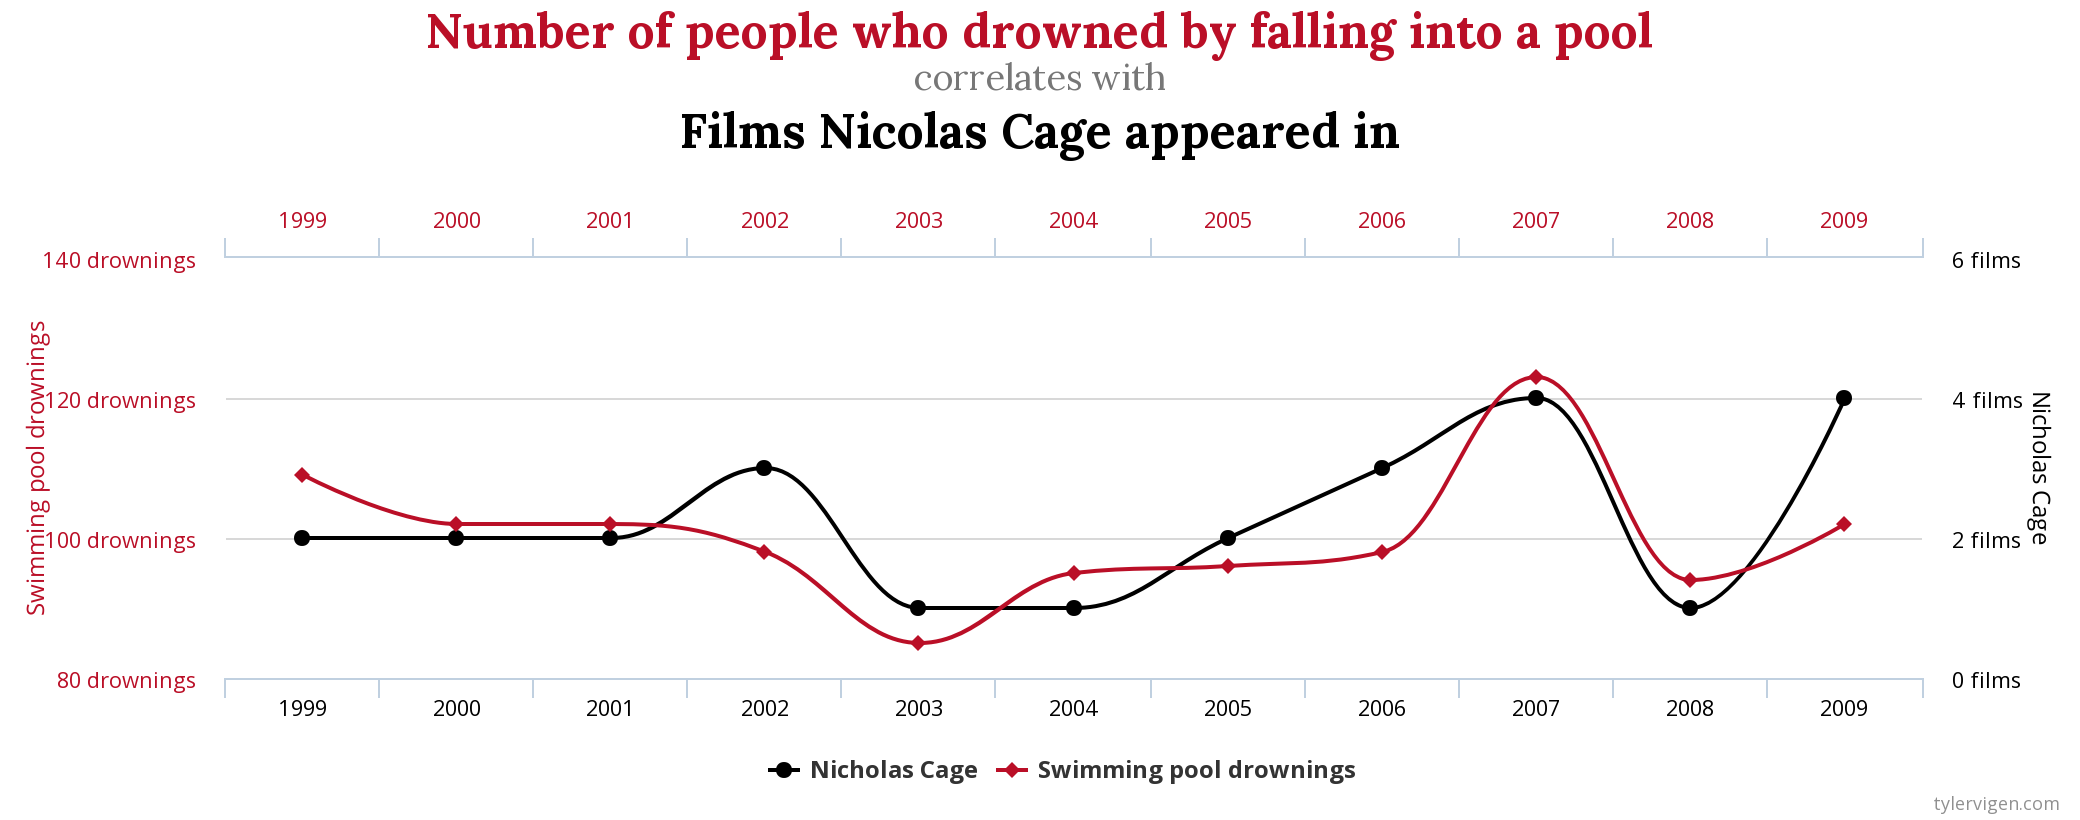
\includegraphics[width=10cm, height=6cm, keepaspectratio]{img/chart.png}  
(source: https://www.tylervigen.com/spurious-correlations)
\end{center}
\newpage

\Large Large letters \footnote{This is a footnote}

\begin{center}\rule{0.5\linewidth}{0.5pt}\end{center}

You may also use the LaTeX citation syntax. We need to specify what
package do we want to use to manage the citations, e.g.:

\texttt{pdf\_document:}\strut \\
\texttt{citation\_package:\ natbib}

\hypertarget{md}{%
\paragraph{MD}\label{md}}

\texttt{Studies\ concerning\ other\ cultural\ goods\ exploit\ quasi-natural\ experiments\ of\ policy\ and\ institutional\ changes.\ One\ example\ of\ the\ policy\ change\ is\ the\ introduction\ of\ download\ penalization\ in\ France\ (HADOPI),\ as\ scrutinized\ by\ \textbackslash{}citet\{danaher\_effect\_2012\}.\ The\ analyzed\ cases\ of\ institutional\ change\ include\ the\ sudden\ and\ transitory\ disappearance\ of\ the\ NBC\ content\ from\ iTunes\ \textbackslash{}citep{[}a\ case\ unrelated\ to\ unauthorized\ distribution,\ hence\ plausibly\ exogenous,\ see{]}{[}{]}\{danaher\_converting\_2010\}\ as\ well\ as\ the\ Megaupload\ shutdown\ \textbackslash{}citep\{danaher\_gone\_2014,peukert\_piracy\_2013\}\ and\ website\ blocking\ in\ the\ UK\ \textbackslash{}citep\{danaher\_website\_2016\}.\ Interestingly,\ \textbackslash{}citet\{danaher\_gone\_2014\}\ and\ \textbackslash{}citet\{peukert\_piracy\_2013\}\ analyzing\ the\ same\ case\ of\ Megaupload\ shutdown\ come\ to\ rather\ different\ conclusions:\ the\ former\ find\ that\ the\ shutdown\ caused\ an\ increase\ in\ digital\ downloads\ from\ legal\ sources;\ the\ latter\ finds\ no\ change\ in\ box\ office\ revenue.\ This\ difference\ could\ be\ attributed\ to\ the\ fact\ that\ a\ downloaded\ "pirated"\ copy\ may\ be\ a\ perfect\ substitute\ for\ a\ copy\ downloaded\ from\ a\ legitimate\ source,\ but\ not\ for\ a\ visit\ to\ the\ movie\ theater.\textbackslash{}footnote\{The\ two\ studies\ \ differ\ also\ methodologically\ and\ in\ the\ sample\ used:\ \textbackslash{}citet\{danaher\_gone\_2014\}\ covering\ 12\ countries\ \textbackslash{}citet\{peukert\_piracy\_2013\}\ as\ many\ as\ 50\ countries.\}\ \textbackslash{}citet\{danaher\_website\_2016\}\ argue\ that\ only\ large\ scale\ interventions\ (such\ as\ blocking\ multiple\ websites\ with\ unauthorized\ distribution)\ appear\ noticeably\ reduce\ "piracy"\ and\ raise\ paid\ consumption,\ but\ these\ effects\ are\ only\ transitory.}

\hypertarget{output}{%
\paragraph{Output}\label{output}}

Studies concerning other cultural goods exploit quasi-natural
experiments of policy and institutional changes. One example of the
policy change is the introduction of download penalization in France
(HADOPI), as scrutinized by \citet{danaher_effect_2012}. The analyzed
cases of institutional change include the sudden and transitory
disappearance of the NBC content from iTunes
\citep[a case unrelated to unauthorized distribution, hence plausibly exogenous, see][]{danaher_converting_2010}
as well as the Megaupload shutdown
\citep{danaher_gone_2014,peukert_piracy_2013} and website blocking in
the UK \citep{danaher_website_2016}. Interestingly,
\citet{danaher_gone_2014} and \citet{peukert_piracy_2013} analyzing the
same case of Megaupload shutdown come to rather different conclusions:
the former find that the shutdown caused an increase in digital
downloads from legal sources; the latter finds no change in box office
revenue. This difference could be attributed to the fact that a
downloaded ``pirated'' copy may be a perfect substitute for a copy
downloaded from a legitimate source, but not for a visit to the movie
theater.\footnote{The two studies  differ also methodologically and in the sample used: \citet{danaher_gone_2014} covering 12 countries \citet{peukert_piracy_2013} as many as 50 countries.}
\citet{danaher_website_2016} argue that only large scale interventions
(such as blocking multiple websites with unauthorized distribution)
appear noticeably reduce ``piracy'' and raise paid consumption, but
these effects are only transitory.

\hypertarget{bibliography}{%
\section{Bibliography}\label{bibliography}}

The cited works get pasted here.

  \bibliography{bibliography.bib}

\end{document}
